% Kapitel 2 - Mathe

\chapter{Mathematische Ausdr�cke und Formeln} \label{chap:math}
%%%%%%%%%%%%%%%%%%%%%%%%%%%%%%%%%%%%%%%%%%%%%%%%%%%%%%%%%%%%%%%%%%%%%%%%%%%%%%%%%%%%%%%%%%%%%%

%%%%%%%%%%%%%%%%%%%%%%%%%%%%%%%%%%%%%%%%%%%%%%%%%%%%%%%%%%%%%%%%%%%%%%%%%%%%%%%%%%%%%%%%%%%%%%
\section{Matrizen} \label{sec:matrizen}

Matrizen gehen so:

Definition einer $(M \times N)$-Matrix:
\begin{equation}
	{\bf A}=\left(
		\begin{array}{cccc}
			a_{11}  & a_{12}        & \cdots                & a_{1N}        \\
			a_{21}  & a_{22}        & \cdots                & a_{2N}        \\
			\vdots  & \vdots        & \ddots                & \vdots        \\
			a_{M1}  & a_{M2}        & \cdots                & a_{MN}        
		\end{array}
		\right)
		  =(a_{ij})
\end{equation}


\section{Schreibweisen und Formelsatz}

Oft stellt sich die Frage, ob man ein Formelzeichen oder einen Bezeichner in einer Zeichnung senkrecht (also ``normal'' bzw. nicht-kursiv) oder \textit{kursiv} zu schreiben hat. Um diese Fragen zu kl�ren folgen nun die wichtigsten Regeln, wie sie Standard sein sollten. Sie sind aus den DIN-Normen 1338 und 1302 �bernommen. Zus�tzlich wird darauf hingewiesen, wie man in mathematischen Formeln die korrekten Abst�nde zwischen den Elementen und Einheiten einzuhalten hat.

Um zwischen mathematischen und physikalischen Konstanten und Variablen unterscheiden zu k�nnen, werden diese mit unterschiedlichen Schreibweisen gekennzeichnet.

\subsection{Senkrechte Schreibweise}
\textbf{Mathematische Konstanten} werden generell senkrecht geschrieben.
Dazu geh�ren beispielsweise die Euler�sche Zahl $\mathrm{e}$, die Zahl $\pi$ oder $	\mathrm{j}$ bzw. $	\mathrm{i} = \sqrt{-1}$. \textbf{Mathematische Funktionen und Operatoren} schreibt man senkrecht.
z.B. $\sin, \cos, \exp, \ln$ und  $\mathrm{\frac{d}{dt}}$

\subsection{Kursive Schreibweise}
\textbf{\textit{Physikalische Konstanten}}, die physikalische Gr��en bezeichnen werden generell \textit{kursiv} geschrieben. 
z.B. $R, L$ oder $i, u$ und Konstanten wie $\epsilon_0$ oder $k$.

\textbf{\textit{Variablen}} werden generell kursiv geschrieben

\subsection{Schreibweise des Index}
F�r Indizes gelten dieselben wie oben beschriebenen Regeln:
Beschreiben die Indizes eine Variable, so werden sie kursiv geschrieben So schreibt man beispielsweise den ohm�schen Widerstand $R$ einer Induktivit�t $L$: $R_L$. $R$ und $L$ bezeichnen beide physikalische Gr��en, und werden somit kursiv geschrieben.
Dient der Index jedoch der Bezeichnung der Funktion von bestimmten Elementen, so wird dieser senkrecht gedruckt. M�chte man beispielsweise einen Widerstand R als Lastwiderstand kennzeichnen, so geschieht dies mit einer senkrechten Indizierung: $R_{\mathrm{Last}}$
Z�hlvariablen, als oft vorkommendes Beispiel, werden als Ver�nderliche im Index ebenfalls kursiv geschrieben. Z.B. $k_n$ , wobei $n$ beispielsweise die Zahlen von $0 bis 10$ durchl�uft.
Ein bestimmtes Element z.B. von einem Vektor, wird jedoch mit senkrechten Zahlen indiziert. So z.B. $k_1$.

Der folgende Hinweis ist eigentlich unn�tig: 
{\footnotesize Hinweis f�r Microsoft Word:
Neben der �blichen Formatierung �ber Men�befehle gibt es noch die M�glichkeit Shortcuts einzusetzen:
Soll ein Index hochgestellt werden, so bet�tigt man unter Festhalten der Ctrl- bzw. Strg- Taste die * - Taste. Jetzt kann man den gew�nschten Index eintippen.
Soll ein Index tiefgestellt werden, so dr�ckt man Ctrl bzw. Strg und \#.}

\section{Formelsatz}
\subsection[Formelabst�nde]{Korrekte Abst�nde in Formeln}
Man nutze z.B. den Befehl ``$\backslash$unit [2]\{kHz\}'': Das Ergebnis sieht dann immer so aus $f_1=\unit[2]{kHz}$. Der folgende Abschnitt er�brigt sich bei Benutzung von Latex. {\footnotesize MS Word: Um Formeln �bersichtlicher zu gestalten, soll zwischen allen Elementen ein festes Leerzeichen, also ein an den vorhergehenden Ausdruck gebundenes Freizeichen gelassen werden. In Microsoft Word und im Formeleditor erh�lt man ein solches Leerzeichen indem man die Space-Taste unter Gedr�ckthalten der Shift und der Ctrl- bzw. Strg-Taste bet�tigt. 
Auf dem Bildschirm werden diese als Steuerzeichen ``$ \circ $'' sichtbar. 
$R = 100 \Omega$  ist als $R \circ = \circ 100 \circ \Omega$zu sehen. Diese Regelung ist besonders bei einheitengebundenen Zahlen wie in diesem Beispiel zu beachten. So muss zwischen Zahl und Einheit immer ein festes Leerzeichen gesetzt werden! Abgesehen von der �bersicht haben diese festen Leerzeichen den Vorteil, dass die Zahlen beim Zeilenumbruch nicht von ihrer Einheit getrennt werden.}

\normalsize
\newpage
\subsection[Formelbeispiel]{Beispiel f�r eine richtig dargestellte Formel}
Als Bild (aus Word):
\begin{figure}[!htbp]
			\begin{center}
				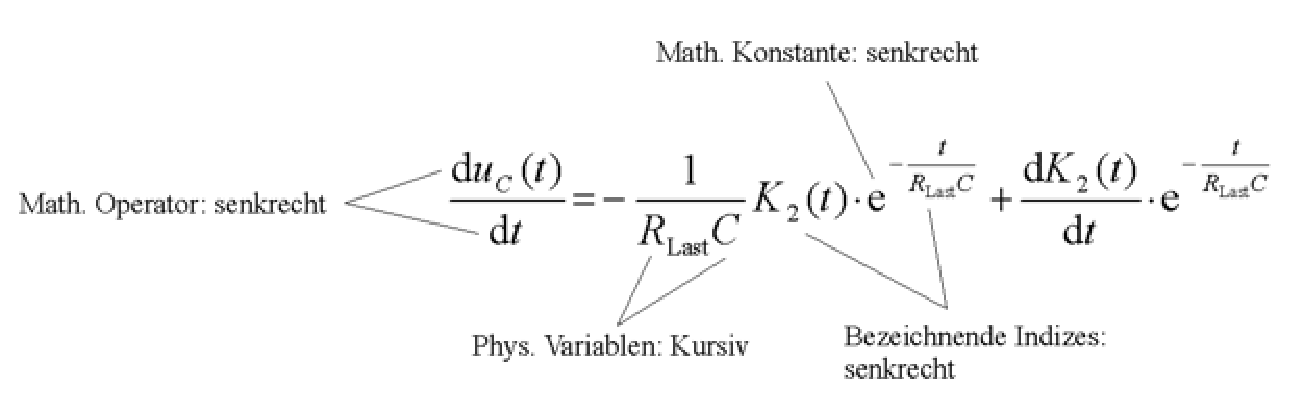
\includegraphics[scale=0.6]{../Kapitel2/Bilder/formelbeispiel.eps}
				\caption{Formelbeispiel}
				\label{kap2:formelbeispiel}
  		\end{center}  
\end{figure}

Und nun in Latex als Formel:
\begin{equation}
		\frac{\mathrm{d}u_C(t)}{\mathrm{d}t} 
		=	- \frac{1}{R_{\mathrm{Last}}C} K_2(t) \cdot \mathrm{e}^{-\frac{t}{R_{\mathrm{Last}}C}} 																	+ \frac{\mathrm{d}K_2(t)}{\mathrm{d}t} \cdot \mathrm{e}^{-\frac{t}{R_{\mathrm{Last}}C}}
		\label{kap2:eqformelbeispiel}
\end{equation}


\subsection{Weitere Formeln} \label{sec:formeln}
\subsubsection{Fouriertransformation}
\paragraph{Analyse}
Die Berechnung der Fouriertransformierten\footnote{So k�nnte eine Fu�note aussehen.} erfolgt mit der Analysegleichung:
\begin{equation}
	F(\mathrm{j}\omega)  = {\cal F}[f(t)] = \int\limits_{-\infty}^{\infty}f(t)\cdot \mathrm{e}^{-\mathrm{j}\omega t}\mathrm{d}t
	\label{analft}
\end{equation}

\paragraph{Synthese}
Die Synthesegleichung der Fouriertransformation lautet:

\begin{equation}
	f(t)  = \frac{1}{2 \pi}\int\limits_{-\infty}^{\infty}F(j \omega) \cdot \mathrm{e}^{\mathrm{j}\omega t}\mathrm{d}\omega
	\label{synthft}
\end{equation}

\subsubsection{weitere Transformationen}
Der mathematische Zusammenhang zwischen einer Zeitfunktion $f(t)$ und ihrer %%@
Laplacetransformierten $F(s)$ ist durch die Analysegleichung definiert:
\begin{equation} 
	F(s) = {\cal L}[f(t)] := \int\limits_{-\infty}^{\infty}f(t)\cdot \mathrm{e}^{-st}\mathrm{d}t 
	\label{anallaplace} 
\end{equation} 
Die komplexe Frequenz $s = \sigma +\mathrm{j}\omega$ wird in einem rechtwinkligen Koordinatensystem, der %%@
Laplace- bzw. $s$-Ebene, dargestellt.


Vielen Dank f�r diese Zusammenstellung der Schreibweisen an Stefan � Bauer und Christian Carstensen, ISEA - RWTH-Aachen